\documentclass[twoside]{book}

% Packages required by doxygen
\usepackage{calc}
\usepackage{doxygen}
\usepackage{graphicx}
\usepackage[utf8]{inputenc}
\usepackage{makeidx}
\usepackage{multicol}
\usepackage{multirow}
\usepackage{textcomp}
\usepackage[table]{xcolor}

% Font selection
\usepackage[T1]{fontenc}
\usepackage{mathptmx}
\usepackage[scaled=.90]{helvet}
\usepackage{courier}
\usepackage{amssymb}
\usepackage{sectsty}
\renewcommand{\familydefault}{\sfdefault}
\allsectionsfont{%
  \fontseries{bc}\selectfont%
  \color{darkgray}%
}
\renewcommand{\DoxyLabelFont}{%
  \fontseries{bc}\selectfont%
  \color{darkgray}%
}

% Page & text layout
\usepackage{geometry}
\geometry{%
  a4paper,%
  top=2.5cm,%
  bottom=2.5cm,%
  left=2.5cm,%
  right=2.5cm%
}
\tolerance=750
\hfuzz=15pt
\hbadness=750
\setlength{\emergencystretch}{15pt}
\setlength{\parindent}{0cm}
\setlength{\parskip}{0.2cm}
\makeatletter
\renewcommand{\paragraph}{%
  \@startsection{paragraph}{4}{0ex}{-1.0ex}{1.0ex}{%
    \normalfont\normalsize\bfseries\SS@parafont%
  }%
}
\renewcommand{\subparagraph}{%
  \@startsection{subparagraph}{5}{0ex}{-1.0ex}{1.0ex}{%
    \normalfont\normalsize\bfseries\SS@subparafont%
  }%
}
\makeatother

% Headers & footers
\usepackage{fancyhdr}
\pagestyle{fancyplain}
\fancyhead[LE]{\fancyplain{}{\bfseries\thepage}}
\fancyhead[CE]{\fancyplain{}{}}
\fancyhead[RE]{\fancyplain{}{\bfseries\leftmark}}
\fancyhead[LO]{\fancyplain{}{\bfseries\rightmark}}
\fancyhead[CO]{\fancyplain{}{}}
\fancyhead[RO]{\fancyplain{}{\bfseries\thepage}}
\fancyfoot[LE]{\fancyplain{}{}}
\fancyfoot[CE]{\fancyplain{}{}}
\fancyfoot[RE]{\fancyplain{}{\bfseries\scriptsize Generated on Wed May 25 2016 20\-:07\-:57 for P\-R\-D\-C Project by Doxygen }}
\fancyfoot[LO]{\fancyplain{}{\bfseries\scriptsize Generated on Wed May 25 2016 20\-:07\-:57 for P\-R\-D\-C Project by Doxygen }}
\fancyfoot[CO]{\fancyplain{}{}}
\fancyfoot[RO]{\fancyplain{}{}}
\renewcommand{\footrulewidth}{0.4pt}
\renewcommand{\chaptermark}[1]{%
  \markboth{#1}{}%
}
\renewcommand{\sectionmark}[1]{%
  \markright{\thesection\ #1}%
}

% Indices & bibliography
\usepackage{natbib}
\usepackage[titles]{tocloft}
\setcounter{tocdepth}{3}
\setcounter{secnumdepth}{5}
\makeindex

% Hyperlinks (required, but should be loaded last)
\usepackage{ifpdf}
\ifpdf
  \usepackage[pdftex,pagebackref=true]{hyperref}
\else
  \usepackage[ps2pdf,pagebackref=true]{hyperref}
\fi
\hypersetup{%
  colorlinks=true,%
  linkcolor=blue,%
  citecolor=blue,%
  unicode%
}

% Custom commands
\newcommand{\clearemptydoublepage}{%
  \newpage{\pagestyle{empty}\cleardoublepage}%
}


%===== C O N T E N T S =====

\begin{document}

% Titlepage & ToC
\hypersetup{pageanchor=false}
\pagenumbering{roman}
\begin{titlepage}
\vspace*{7cm}
\begin{center}%
{\Large P\-R\-D\-C Project }\\
\vspace*{1cm}
{\large Generated by Doxygen 1.8.6}\\
\vspace*{0.5cm}
{\small Wed May 25 2016 20:07:57}\\
\end{center}
\end{titlepage}
\clearemptydoublepage
\tableofcontents
\clearemptydoublepage
\pagenumbering{arabic}
\hypersetup{pageanchor=true}

%--- Begin generated contents ---
\chapter{Namespace Index}
\section{Namespace List}
Here is a list of all namespaces with brief descriptions\-:\begin{DoxyCompactList}
\item\contentsline{section}{\hyperlink{namespaceprdc__lzw}{prdc\-\_\-lzw} \\*P\-R\-D\-Cで用いる\-L\-Z\-W圧縮に関する名前空間 }{\pageref{namespaceprdc__lzw}}{}
\item\contentsline{section}{\hyperlink{namespaceprdc__util}{prdc\-\_\-util} }{\pageref{namespaceprdc__util}}{}
\end{DoxyCompactList}

\chapter{Class Index}
\section{Class List}
Here are the classes, structs, unions and interfaces with brief descriptions\-:\begin{DoxyCompactList}
\item\contentsline{section}{\hyperlink{classprdc__lzw_1_1Dictionary}{prdc\-\_\-lzw\-::\-Dictionary} \\*L\-Z\-W辞書クラス }{\pageref{classprdc__lzw_1_1Dictionary}}{}
\item\contentsline{section}{\hyperlink{classprdc__lzw_1_1LzwNode}{prdc\-\_\-lzw\-::\-Lzw\-Node} \\*L\-Z\-W辞書のノード }{\pageref{classprdc__lzw_1_1LzwNode}}{}
\end{DoxyCompactList}

\chapter{File Index}
\section{File List}
Here is a list of all files with brief descriptions\-:\begin{DoxyCompactList}
\item\contentsline{section}{src/\hyperlink{Dictionary_8cpp}{Dictionary.\-cpp} \\*辞書クラスの実装 }{\pageref{Dictionary_8cpp}}{}
\item\contentsline{section}{src/\hyperlink{Dictionary_8h}{Dictionary.\-h} \\*L\-Z\-W辞書クラス定義ファイル }{\pageref{Dictionary_8h}}{}
\item\contentsline{section}{src/\hyperlink{main_8cpp}{main.\-cpp} }{\pageref{main_8cpp}}{}
\item\contentsline{section}{src/\hyperlink{util_8cpp}{util.\-cpp} }{\pageref{util_8cpp}}{}
\item\contentsline{section}{src/\hyperlink{util_8h}{util.\-h} }{\pageref{util_8h}}{}
\end{DoxyCompactList}

\chapter{Namespace Documentation}
\hypertarget{namespaceprdc__lzw}{\section{prdc\-\_\-lzw Namespace Reference}
\label{namespaceprdc__lzw}\index{prdc\-\_\-lzw@{prdc\-\_\-lzw}}
}


P\-R\-D\-Cで用いる\-L\-Z\-W圧縮に関する名前空間  


\subsection*{Classes}
\begin{DoxyCompactItemize}
\item 
class \hyperlink{classprdc__lzw_1_1LzwNode}{Lzw\-Node}
\begin{DoxyCompactList}\small\item\em L\-Z\-W辞書のノード \end{DoxyCompactList}\item 
class \hyperlink{classprdc__lzw_1_1Dictionary}{Dictionary}
\begin{DoxyCompactList}\small\item\em L\-Z\-W辞書クラス \end{DoxyCompactList}\end{DoxyCompactItemize}
\subsection*{Functions}
\begin{DoxyCompactItemize}
\item 
void \hyperlink{namespaceprdc__lzw_a09931e4cc68e675f2058ee251b1e761f}{compress} (const std\-::string \&uncompressed, std\-::vector$<$ int $>$ \&compressed, \hyperlink{classprdc__lzw_1_1Dictionary}{Dictionary} \&output\-\_\-dic)
\begin{DoxyCompactList}\small\item\em 文字列を圧縮し、辞書を抽出する \end{DoxyCompactList}\item 
void \hyperlink{namespaceprdc__lzw_a81663f550046c9a805ca2e4d60df03dc}{compress\-\_\-with\-\_\-outer\-\_\-dictionary} (const std\-::string \&uncompressed, std\-::vector$<$ int $>$ \&compressed, \hyperlink{classprdc__lzw_1_1Dictionary}{Dictionary} \&output\-\_\-dic)
\end{DoxyCompactItemize}


\subsection{Detailed Description}
P\-R\-D\-Cで用いる\-L\-Z\-W圧縮に関する名前空間 

\subsection{Function Documentation}
\hypertarget{namespaceprdc__lzw_a09931e4cc68e675f2058ee251b1e761f}{\index{prdc\-\_\-lzw@{prdc\-\_\-lzw}!compress@{compress}}
\index{compress@{compress}!prdc_lzw@{prdc\-\_\-lzw}}
\subsubsection[{compress}]{\setlength{\rightskip}{0pt plus 5cm}void prdc\-\_\-lzw\-::compress (
\begin{DoxyParamCaption}
\item[{const std\-::string \&}]{uncompressed, }
\item[{std\-::vector$<$ int $>$ \&}]{compressed, }
\item[{Dictionary \&}]{output\-\_\-dic}
\end{DoxyParamCaption}
)}}\label{namespaceprdc__lzw_a09931e4cc68e675f2058ee251b1e761f}


文字列を圧縮し、辞書を抽出する 


\begin{DoxyParams}{Parameters}
{\em uncompressed} & 圧縮する文字列 \\
\hline
{\em compressed} & 圧縮された文字列(数値) \\
\hline
{\em output\-\_\-dic} & 出力される辞書 \\
\hline
\end{DoxyParams}


Definition at line 14 of file Lzw.\-cpp.



References prdc\-\_\-lzw\-::\-Dictionary\-::\-Add\-Node(), prdc\-\_\-lzw\-::\-Lzw\-Node\-::\-Find\-Child(), prdc\-\_\-lzw\-::\-Lzw\-Node\-::get\-Data(), and prdc\-\_\-lzw\-::\-Dictionary\-::get\-Root().



Referenced by main().

\hypertarget{namespaceprdc__lzw_a81663f550046c9a805ca2e4d60df03dc}{\index{prdc\-\_\-lzw@{prdc\-\_\-lzw}!compress\-\_\-with\-\_\-outer\-\_\-dictionary@{compress\-\_\-with\-\_\-outer\-\_\-dictionary}}
\index{compress\-\_\-with\-\_\-outer\-\_\-dictionary@{compress\-\_\-with\-\_\-outer\-\_\-dictionary}!prdc_lzw@{prdc\-\_\-lzw}}
\subsubsection[{compress\-\_\-with\-\_\-outer\-\_\-dictionary}]{\setlength{\rightskip}{0pt plus 5cm}void prdc\-\_\-lzw\-::compress\-\_\-with\-\_\-outer\-\_\-dictionary (
\begin{DoxyParamCaption}
\item[{const std\-::string \&}]{uncompressed, }
\item[{std\-::vector$<$ int $>$ \&}]{compressed, }
\item[{Dictionary \&}]{output\-\_\-dic}
\end{DoxyParamCaption}
)}}\label{namespaceprdc__lzw_a81663f550046c9a805ca2e4d60df03dc}


Definition at line 36 of file Lzw.\-cpp.


\input{namespaceprdc__util}
\chapter{Class Documentation}
\hypertarget{classprdc__lzw_1_1Dictionary}{\section{prdc\-\_\-lzw\-:\-:Dictionary Class Reference}
\label{classprdc__lzw_1_1Dictionary}\index{prdc\-\_\-lzw\-::\-Dictionary@{prdc\-\_\-lzw\-::\-Dictionary}}
}


L\-Z\-W辞書クラス  




{\ttfamily \#include $<$Dictionary.\-h$>$}



Collaboration diagram for prdc\-\_\-lzw\-:\-:Dictionary\-:\nopagebreak
\begin{figure}[H]
\begin{center}
\leavevmode
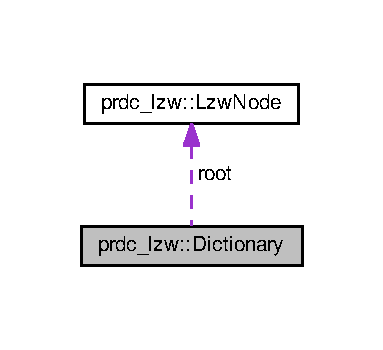
\includegraphics[width=184pt]{classprdc__lzw_1_1Dictionary__coll__graph}
\end{center}
\end{figure}
\subsection*{Public Member Functions}
\begin{DoxyCompactItemize}
\item 
\hyperlink{classprdc__lzw_1_1Dictionary_a7a53efd7967e59748f321938aa983368}{Dictionary} ()
\item 
virtual \hyperlink{classprdc__lzw_1_1Dictionary_a953fce0e9128a8e48b62779fdefcc051}{$\sim$\-Dictionary} ()
\item 
\hyperlink{classprdc__lzw_1_1LzwNode}{Lzw\-Node} $\ast$ \hyperlink{classprdc__lzw_1_1Dictionary_a4ac9a03c8ead8d6ca17e080ff9227fd9}{get\-Root} ()
\item 
void \hyperlink{classprdc__lzw_1_1Dictionary_ad9a68c58a75d9eec5eb2aaf528b9fbe4}{Add\-Node} (\hyperlink{classprdc__lzw_1_1LzwNode}{Lzw\-Node} $\ast$node, char key\-\_\-word)
\begin{DoxyCompactList}\small\item\em 辞書中の指定したノードに文字を追加する \end{DoxyCompactList}\item 
\hyperlink{classprdc__lzw_1_1LzwNode}{Lzw\-Node} $\ast$ \hyperlink{classprdc__lzw_1_1Dictionary_ac5577ef2e482e191a0b6376e28564b7e}{Search\-Node} (std\-::string key\-\_\-word)
\begin{DoxyCompactList}\small\item\em key\-\_\-wordのノードを辞書から検索し返す。 \end{DoxyCompactList}\end{DoxyCompactItemize}
\subsection*{Private Attributes}
\begin{DoxyCompactItemize}
\item 
int \hyperlink{classprdc__lzw_1_1Dictionary_ac96b4db6d4692ba9b082fe32e54bcf0d}{dict\-\_\-size}
\begin{DoxyCompactList}\small\item\em 辞書に単語がいくつ登録されているか(辞書番号をつける際に利用) \end{DoxyCompactList}\item 
\hyperlink{classprdc__lzw_1_1LzwNode}{Lzw\-Node} $\ast$ \hyperlink{classprdc__lzw_1_1Dictionary_a95b84d2d9ebb6277cfc6bffba5dee738}{root}
\end{DoxyCompactItemize}


\subsection{Detailed Description}
L\-Z\-W辞書クラス 

文字列の登録と検索ができる \begin{DoxyAuthor}{Author}
uchino 
\end{DoxyAuthor}


Definition at line 60 of file Dictionary.\-h.



\subsection{Constructor \& Destructor Documentation}
\hypertarget{classprdc__lzw_1_1Dictionary_a7a53efd7967e59748f321938aa983368}{\index{prdc\-\_\-lzw\-::\-Dictionary@{prdc\-\_\-lzw\-::\-Dictionary}!Dictionary@{Dictionary}}
\index{Dictionary@{Dictionary}!prdc_lzw::Dictionary@{prdc\-\_\-lzw\-::\-Dictionary}}
\subsubsection[{Dictionary}]{\setlength{\rightskip}{0pt plus 5cm}prdc\-\_\-lzw\-::\-Dictionary\-::\-Dictionary (
\begin{DoxyParamCaption}
{}
\end{DoxyParamCaption}
)}}\label{classprdc__lzw_1_1Dictionary_a7a53efd7967e59748f321938aa983368}


Definition at line 41 of file Dictionary.\-cpp.



References prdc\-\_\-lzw\-::\-Lzw\-Node\-::children, and root.

\hypertarget{classprdc__lzw_1_1Dictionary_a953fce0e9128a8e48b62779fdefcc051}{\index{prdc\-\_\-lzw\-::\-Dictionary@{prdc\-\_\-lzw\-::\-Dictionary}!$\sim$\-Dictionary@{$\sim$\-Dictionary}}
\index{$\sim$\-Dictionary@{$\sim$\-Dictionary}!prdc_lzw::Dictionary@{prdc\-\_\-lzw\-::\-Dictionary}}
\subsubsection[{$\sim$\-Dictionary}]{\setlength{\rightskip}{0pt plus 5cm}prdc\-\_\-lzw\-::\-Dictionary\-::$\sim$\-Dictionary (
\begin{DoxyParamCaption}
{}
\end{DoxyParamCaption}
)\hspace{0.3cm}{\ttfamily [virtual]}}}\label{classprdc__lzw_1_1Dictionary_a953fce0e9128a8e48b62779fdefcc051}


Definition at line 51 of file Dictionary.\-cpp.



References root.



\subsection{Member Function Documentation}
\hypertarget{classprdc__lzw_1_1Dictionary_ad9a68c58a75d9eec5eb2aaf528b9fbe4}{\index{prdc\-\_\-lzw\-::\-Dictionary@{prdc\-\_\-lzw\-::\-Dictionary}!Add\-Node@{Add\-Node}}
\index{Add\-Node@{Add\-Node}!prdc_lzw::Dictionary@{prdc\-\_\-lzw\-::\-Dictionary}}
\subsubsection[{Add\-Node}]{\setlength{\rightskip}{0pt plus 5cm}void prdc\-\_\-lzw\-::\-Dictionary\-::\-Add\-Node (
\begin{DoxyParamCaption}
\item[{{\bf Lzw\-Node} $\ast$}]{node, }
\item[{char}]{key\-\_\-word}
\end{DoxyParamCaption}
)}}\label{classprdc__lzw_1_1Dictionary_ad9a68c58a75d9eec5eb2aaf528b9fbe4}


辞書中の指定したノードに文字を追加する 


\begin{DoxyParams}{Parameters}
{\em key\-\_\-word} & 追加する文字 \\
\hline
{\em node} & 文字を追加するノード \\
\hline
\end{DoxyParams}
\begin{DoxyNote}{Note}
辞書番号の管理のため直接ノードに子を追加させない 
\end{DoxyNote}


Definition at line 55 of file Dictionary.\-cpp.



References dict\-\_\-size, and prdc\-\_\-lzw\-::\-Lzw\-Node\-::\-Insert\-Child().



Referenced by prdc\-\_\-lzw\-::compress().

\hypertarget{classprdc__lzw_1_1Dictionary_a4ac9a03c8ead8d6ca17e080ff9227fd9}{\index{prdc\-\_\-lzw\-::\-Dictionary@{prdc\-\_\-lzw\-::\-Dictionary}!get\-Root@{get\-Root}}
\index{get\-Root@{get\-Root}!prdc_lzw::Dictionary@{prdc\-\_\-lzw\-::\-Dictionary}}
\subsubsection[{get\-Root}]{\setlength{\rightskip}{0pt plus 5cm}{\bf Lzw\-Node}$\ast$ prdc\-\_\-lzw\-::\-Dictionary\-::get\-Root (
\begin{DoxyParamCaption}
{}
\end{DoxyParamCaption}
)\hspace{0.3cm}{\ttfamily [inline]}}}\label{classprdc__lzw_1_1Dictionary_a4ac9a03c8ead8d6ca17e080ff9227fd9}


Definition at line 64 of file Dictionary.\-h.



References root.



Referenced by prdc\-\_\-lzw\-::compress().

\hypertarget{classprdc__lzw_1_1Dictionary_ac5577ef2e482e191a0b6376e28564b7e}{\index{prdc\-\_\-lzw\-::\-Dictionary@{prdc\-\_\-lzw\-::\-Dictionary}!Search\-Node@{Search\-Node}}
\index{Search\-Node@{Search\-Node}!prdc_lzw::Dictionary@{prdc\-\_\-lzw\-::\-Dictionary}}
\subsubsection[{Search\-Node}]{\setlength{\rightskip}{0pt plus 5cm}{\bf Lzw\-Node}$\ast$ prdc\-\_\-lzw\-::\-Dictionary\-::\-Search\-Node (
\begin{DoxyParamCaption}
\item[{std\-::string}]{key\-\_\-word}
\end{DoxyParamCaption}
)}}\label{classprdc__lzw_1_1Dictionary_ac5577ef2e482e191a0b6376e28564b7e}


key\-\_\-wordのノードを辞書から検索し返す。 


\begin{DoxyParams}{Parameters}
{\em key\-\_\-word} & 検索する文字列 \\
\hline
\end{DoxyParams}
\begin{DoxyReturn}{Returns}
key\-\_\-wordのノード。辞書中に存在しなければ\-N\-U\-L\-Lを返す 
\end{DoxyReturn}


\subsection{Member Data Documentation}
\hypertarget{classprdc__lzw_1_1Dictionary_ac96b4db6d4692ba9b082fe32e54bcf0d}{\index{prdc\-\_\-lzw\-::\-Dictionary@{prdc\-\_\-lzw\-::\-Dictionary}!dict\-\_\-size@{dict\-\_\-size}}
\index{dict\-\_\-size@{dict\-\_\-size}!prdc_lzw::Dictionary@{prdc\-\_\-lzw\-::\-Dictionary}}
\subsubsection[{dict\-\_\-size}]{\setlength{\rightskip}{0pt plus 5cm}int prdc\-\_\-lzw\-::\-Dictionary\-::dict\-\_\-size\hspace{0.3cm}{\ttfamily [private]}}}\label{classprdc__lzw_1_1Dictionary_ac96b4db6d4692ba9b082fe32e54bcf0d}


辞書に単語がいくつ登録されているか(辞書番号をつける際に利用) 



Definition at line 85 of file Dictionary.\-h.



Referenced by Add\-Node().

\hypertarget{classprdc__lzw_1_1Dictionary_a95b84d2d9ebb6277cfc6bffba5dee738}{\index{prdc\-\_\-lzw\-::\-Dictionary@{prdc\-\_\-lzw\-::\-Dictionary}!root@{root}}
\index{root@{root}!prdc_lzw::Dictionary@{prdc\-\_\-lzw\-::\-Dictionary}}
\subsubsection[{root}]{\setlength{\rightskip}{0pt plus 5cm}{\bf Lzw\-Node}$\ast$ prdc\-\_\-lzw\-::\-Dictionary\-::root\hspace{0.3cm}{\ttfamily [private]}}}\label{classprdc__lzw_1_1Dictionary_a95b84d2d9ebb6277cfc6bffba5dee738}


Definition at line 86 of file Dictionary.\-h.



Referenced by Dictionary(), get\-Root(), and $\sim$\-Dictionary().



The documentation for this class was generated from the following files\-:\begin{DoxyCompactItemize}
\item 
src/\hyperlink{Dictionary_8h}{Dictionary.\-h}\item 
src/\hyperlink{Dictionary_8cpp}{Dictionary.\-cpp}\end{DoxyCompactItemize}

\hypertarget{classprdc__lzw_1_1LzwNode}{\section{prdc\-\_\-lzw\-:\-:Lzw\-Node Class Reference}
\label{classprdc__lzw_1_1LzwNode}\index{prdc\-\_\-lzw\-::\-Lzw\-Node@{prdc\-\_\-lzw\-::\-Lzw\-Node}}
}


L\-Z\-W辞書のノード  




{\ttfamily \#include $<$Dictionary.\-h$>$}

\subsection*{Public Member Functions}
\begin{DoxyCompactItemize}
\item 
int \hyperlink{classprdc__lzw_1_1LzwNode_a43acbf6c83a319186feb5ff239e6714d}{get\-\_\-data} ()
\item 
char \hyperlink{classprdc__lzw_1_1LzwNode_afb7e80f3c9f742548fa9e82b4236ae36}{get\-\_\-content} ()
\item 
\hyperlink{classprdc__lzw_1_1LzwNode}{Lzw\-Node} $\ast$ \hyperlink{classprdc__lzw_1_1LzwNode_a4dbccb5fb97eae6f622a66a53eda46a3}{Find\-Child} (char c)
\begin{DoxyCompactList}\small\item\em 文字cを子供に持っていればそれを返す \end{DoxyCompactList}\end{DoxyCompactItemize}
\subsection*{Public Attributes}
\begin{DoxyCompactItemize}
\item 
std\-::vector$<$ \hyperlink{classprdc__lzw_1_1LzwNode}{Lzw\-Node} $\ast$ $>$ \hyperlink{classprdc__lzw_1_1LzwNode_abc56c04f0b0f97baf8e2b3f08d736463}{children}
\end{DoxyCompactItemize}
\subsection*{Private Member Functions}
\begin{DoxyCompactItemize}
\item 
\hyperlink{classprdc__lzw_1_1LzwNode_aecd8429cfcb52da0c5a88c2eb2ce8f17}{Lzw\-Node} ()
\begin{DoxyCompactList}\small\item\em 子ノード \end{DoxyCompactList}\item 
\hyperlink{classprdc__lzw_1_1LzwNode_ab376216cc0c3c4893de9cc82e193bc0a}{Lzw\-Node} (int d, char c)
\item 
virtual \hyperlink{classprdc__lzw_1_1LzwNode_ab7c9e93839328025287d465734dfba4a}{$\sim$\-Lzw\-Node} ()
\item 
void \hyperlink{classprdc__lzw_1_1LzwNode_adcb9f453effcb8fac95bb08a59665eb7}{Insert\-Child} (int \hyperlink{classprdc__lzw_1_1LzwNode_ac85178681ea1181b22c3ac43af32515a}{data}, char c)
\begin{DoxyCompactList}\small\item\em 子ノードの挿入 \end{DoxyCompactList}\end{DoxyCompactItemize}
\subsection*{Private Attributes}
\begin{DoxyCompactItemize}
\item 
int \hyperlink{classprdc__lzw_1_1LzwNode_ac85178681ea1181b22c3ac43af32515a}{data}
\item 
char \hyperlink{classprdc__lzw_1_1LzwNode_acb2b7cb34053125cfdf7595aba9bc172}{content}
\begin{DoxyCompactList}\small\item\em 辞書番号 \end{DoxyCompactList}\end{DoxyCompactItemize}
\subsection*{Friends}
\begin{DoxyCompactItemize}
\item 
class \hyperlink{classprdc__lzw_1_1LzwNode_a61780a02d5e0994eb40a4b79f9c007ad}{Dictionary}
\end{DoxyCompactItemize}


\subsection{Detailed Description}
L\-Z\-W辞書のノード 

内部に辞書番号(辞書に何個目に追加されたか)と単語(検索用)を持つ 

Definition at line 26 of file Dictionary.\-h.



\subsection{Constructor \& Destructor Documentation}
\hypertarget{classprdc__lzw_1_1LzwNode_aecd8429cfcb52da0c5a88c2eb2ce8f17}{\index{prdc\-\_\-lzw\-::\-Lzw\-Node@{prdc\-\_\-lzw\-::\-Lzw\-Node}!Lzw\-Node@{Lzw\-Node}}
\index{Lzw\-Node@{Lzw\-Node}!prdc_lzw::LzwNode@{prdc\-\_\-lzw\-::\-Lzw\-Node}}
\subsubsection[{Lzw\-Node}]{\setlength{\rightskip}{0pt plus 5cm}prdc\-\_\-lzw\-::\-Lzw\-Node\-::\-Lzw\-Node (
\begin{DoxyParamCaption}
{}
\end{DoxyParamCaption}
)\hspace{0.3cm}{\ttfamily [private]}}}\label{classprdc__lzw_1_1LzwNode_aecd8429cfcb52da0c5a88c2eb2ce8f17}


子ノード 



Definition at line 17 of file Dictionary.\-cpp.



Referenced by Insert\-Child().

\hypertarget{classprdc__lzw_1_1LzwNode_ab376216cc0c3c4893de9cc82e193bc0a}{\index{prdc\-\_\-lzw\-::\-Lzw\-Node@{prdc\-\_\-lzw\-::\-Lzw\-Node}!Lzw\-Node@{Lzw\-Node}}
\index{Lzw\-Node@{Lzw\-Node}!prdc_lzw::LzwNode@{prdc\-\_\-lzw\-::\-Lzw\-Node}}
\subsubsection[{Lzw\-Node}]{\setlength{\rightskip}{0pt plus 5cm}prdc\-\_\-lzw\-::\-Lzw\-Node\-::\-Lzw\-Node (
\begin{DoxyParamCaption}
\item[{int}]{d, }
\item[{char}]{c}
\end{DoxyParamCaption}
)\hspace{0.3cm}{\ttfamily [private]}}}\label{classprdc__lzw_1_1LzwNode_ab376216cc0c3c4893de9cc82e193bc0a}


Definition at line 20 of file Dictionary.\-cpp.

\hypertarget{classprdc__lzw_1_1LzwNode_ab7c9e93839328025287d465734dfba4a}{\index{prdc\-\_\-lzw\-::\-Lzw\-Node@{prdc\-\_\-lzw\-::\-Lzw\-Node}!$\sim$\-Lzw\-Node@{$\sim$\-Lzw\-Node}}
\index{$\sim$\-Lzw\-Node@{$\sim$\-Lzw\-Node}!prdc_lzw::LzwNode@{prdc\-\_\-lzw\-::\-Lzw\-Node}}
\subsubsection[{$\sim$\-Lzw\-Node}]{\setlength{\rightskip}{0pt plus 5cm}prdc\-\_\-lzw\-::\-Lzw\-Node\-::$\sim$\-Lzw\-Node (
\begin{DoxyParamCaption}
{}
\end{DoxyParamCaption}
)\hspace{0.3cm}{\ttfamily [private]}, {\ttfamily [virtual]}}}\label{classprdc__lzw_1_1LzwNode_ab7c9e93839328025287d465734dfba4a}


Definition at line 24 of file Dictionary.\-cpp.



References children.



\subsection{Member Function Documentation}
\hypertarget{classprdc__lzw_1_1LzwNode_a4dbccb5fb97eae6f622a66a53eda46a3}{\index{prdc\-\_\-lzw\-::\-Lzw\-Node@{prdc\-\_\-lzw\-::\-Lzw\-Node}!Find\-Child@{Find\-Child}}
\index{Find\-Child@{Find\-Child}!prdc_lzw::LzwNode@{prdc\-\_\-lzw\-::\-Lzw\-Node}}
\subsubsection[{Find\-Child}]{\setlength{\rightskip}{0pt plus 5cm}{\bf Lzw\-Node} $\ast$ prdc\-\_\-lzw\-::\-Lzw\-Node\-::\-Find\-Child (
\begin{DoxyParamCaption}
\item[{char}]{c}
\end{DoxyParamCaption}
)}}\label{classprdc__lzw_1_1LzwNode_a4dbccb5fb97eae6f622a66a53eda46a3}


文字cを子供に持っていればそれを返す 


\begin{DoxyParams}{Parameters}
{\em c} & 探索したい文字 \\
\hline
\end{DoxyParams}
\begin{DoxyReturn}{Returns}
存在すればノードのポインタ、なければ\-N\-U\-L\-L 
\end{DoxyReturn}


Definition at line 30 of file Dictionary.\-cpp.



References children, and content.



Referenced by prdc\-\_\-lzw\-::\-Dictionary\-::\-Compress(), and prdc\-\_\-lzw\-::\-Dictionary\-::\-Search\-Node().

\hypertarget{classprdc__lzw_1_1LzwNode_afb7e80f3c9f742548fa9e82b4236ae36}{\index{prdc\-\_\-lzw\-::\-Lzw\-Node@{prdc\-\_\-lzw\-::\-Lzw\-Node}!get\-\_\-content@{get\-\_\-content}}
\index{get\-\_\-content@{get\-\_\-content}!prdc_lzw::LzwNode@{prdc\-\_\-lzw\-::\-Lzw\-Node}}
\subsubsection[{get\-\_\-content}]{\setlength{\rightskip}{0pt plus 5cm}char prdc\-\_\-lzw\-::\-Lzw\-Node\-::get\-\_\-content (
\begin{DoxyParamCaption}
{}
\end{DoxyParamCaption}
)\hspace{0.3cm}{\ttfamily [inline]}}}\label{classprdc__lzw_1_1LzwNode_afb7e80f3c9f742548fa9e82b4236ae36}


Definition at line 32 of file Dictionary.\-h.



References content.

\hypertarget{classprdc__lzw_1_1LzwNode_a43acbf6c83a319186feb5ff239e6714d}{\index{prdc\-\_\-lzw\-::\-Lzw\-Node@{prdc\-\_\-lzw\-::\-Lzw\-Node}!get\-\_\-data@{get\-\_\-data}}
\index{get\-\_\-data@{get\-\_\-data}!prdc_lzw::LzwNode@{prdc\-\_\-lzw\-::\-Lzw\-Node}}
\subsubsection[{get\-\_\-data}]{\setlength{\rightskip}{0pt plus 5cm}int prdc\-\_\-lzw\-::\-Lzw\-Node\-::get\-\_\-data (
\begin{DoxyParamCaption}
{}
\end{DoxyParamCaption}
)\hspace{0.3cm}{\ttfamily [inline]}}}\label{classprdc__lzw_1_1LzwNode_a43acbf6c83a319186feb5ff239e6714d}


Definition at line 29 of file Dictionary.\-h.



References data.



Referenced by prdc\-\_\-lzw\-::\-Dictionary\-::\-Compress().

\hypertarget{classprdc__lzw_1_1LzwNode_adcb9f453effcb8fac95bb08a59665eb7}{\index{prdc\-\_\-lzw\-::\-Lzw\-Node@{prdc\-\_\-lzw\-::\-Lzw\-Node}!Insert\-Child@{Insert\-Child}}
\index{Insert\-Child@{Insert\-Child}!prdc_lzw::LzwNode@{prdc\-\_\-lzw\-::\-Lzw\-Node}}
\subsubsection[{Insert\-Child}]{\setlength{\rightskip}{0pt plus 5cm}void prdc\-\_\-lzw\-::\-Lzw\-Node\-::\-Insert\-Child (
\begin{DoxyParamCaption}
\item[{int}]{data, }
\item[{char}]{c}
\end{DoxyParamCaption}
)\hspace{0.3cm}{\ttfamily [private]}}}\label{classprdc__lzw_1_1LzwNode_adcb9f453effcb8fac95bb08a59665eb7}


子ノードの挿入 

\begin{DoxyNote}{Note}
辞書クラスからのみ呼び出される\par
(外部から直接子ノードを挿入させない) 
\end{DoxyNote}

\begin{DoxyParams}{Parameters}
{\em data} & 辞書番号 \\
\hline
{\em c} & 格納文字 \\
\hline
\end{DoxyParams}


Definition at line 40 of file Dictionary.\-cpp.



References children, and Lzw\-Node().



Referenced by prdc\-\_\-lzw\-::\-Dictionary\-::\-Add\-Node().



\subsection{Friends And Related Function Documentation}
\hypertarget{classprdc__lzw_1_1LzwNode_a61780a02d5e0994eb40a4b79f9c007ad}{\index{prdc\-\_\-lzw\-::\-Lzw\-Node@{prdc\-\_\-lzw\-::\-Lzw\-Node}!Dictionary@{Dictionary}}
\index{Dictionary@{Dictionary}!prdc_lzw::LzwNode@{prdc\-\_\-lzw\-::\-Lzw\-Node}}
\subsubsection[{Dictionary}]{\setlength{\rightskip}{0pt plus 5cm}friend class {\bf Dictionary}\hspace{0.3cm}{\ttfamily [friend]}}}\label{classprdc__lzw_1_1LzwNode_a61780a02d5e0994eb40a4b79f9c007ad}


Definition at line 27 of file Dictionary.\-h.



\subsection{Member Data Documentation}
\hypertarget{classprdc__lzw_1_1LzwNode_abc56c04f0b0f97baf8e2b3f08d736463}{\index{prdc\-\_\-lzw\-::\-Lzw\-Node@{prdc\-\_\-lzw\-::\-Lzw\-Node}!children@{children}}
\index{children@{children}!prdc_lzw::LzwNode@{prdc\-\_\-lzw\-::\-Lzw\-Node}}
\subsubsection[{children}]{\setlength{\rightskip}{0pt plus 5cm}std\-::vector$<${\bf Lzw\-Node}$\ast$$>$ prdc\-\_\-lzw\-::\-Lzw\-Node\-::children}}\label{classprdc__lzw_1_1LzwNode_abc56c04f0b0f97baf8e2b3f08d736463}


Definition at line 42 of file Dictionary.\-h.



Referenced by prdc\-\_\-lzw\-::\-Dictionary\-::\-Dictionary(), Find\-Child(), Insert\-Child(), and $\sim$\-Lzw\-Node().

\hypertarget{classprdc__lzw_1_1LzwNode_acb2b7cb34053125cfdf7595aba9bc172}{\index{prdc\-\_\-lzw\-::\-Lzw\-Node@{prdc\-\_\-lzw\-::\-Lzw\-Node}!content@{content}}
\index{content@{content}!prdc_lzw::LzwNode@{prdc\-\_\-lzw\-::\-Lzw\-Node}}
\subsubsection[{content}]{\setlength{\rightskip}{0pt plus 5cm}char prdc\-\_\-lzw\-::\-Lzw\-Node\-::content\hspace{0.3cm}{\ttfamily [private]}}}\label{classprdc__lzw_1_1LzwNode_acb2b7cb34053125cfdf7595aba9bc172}


辞書番号 



Definition at line 58 of file Dictionary.\-h.



Referenced by Find\-Child(), and get\-\_\-content().

\hypertarget{classprdc__lzw_1_1LzwNode_ac85178681ea1181b22c3ac43af32515a}{\index{prdc\-\_\-lzw\-::\-Lzw\-Node@{prdc\-\_\-lzw\-::\-Lzw\-Node}!data@{data}}
\index{data@{data}!prdc_lzw::LzwNode@{prdc\-\_\-lzw\-::\-Lzw\-Node}}
\subsubsection[{data}]{\setlength{\rightskip}{0pt plus 5cm}int prdc\-\_\-lzw\-::\-Lzw\-Node\-::data\hspace{0.3cm}{\ttfamily [private]}}}\label{classprdc__lzw_1_1LzwNode_ac85178681ea1181b22c3ac43af32515a}


Definition at line 57 of file Dictionary.\-h.



Referenced by get\-\_\-data().



The documentation for this class was generated from the following files\-:\begin{DoxyCompactItemize}
\item 
src/\hyperlink{Dictionary_8h}{Dictionary.\-h}\item 
src/\hyperlink{Dictionary_8cpp}{Dictionary.\-cpp}\end{DoxyCompactItemize}

\chapter{File Documentation}
\hypertarget{Dictionary_8cpp}{\section{src/\-Dictionary.cpp File Reference}
\label{Dictionary_8cpp}\index{src/\-Dictionary.\-cpp@{src/\-Dictionary.\-cpp}}
}


辞書クラスの実装  


{\ttfamily \#include \char`\"{}Dictionary.\-h\char`\"{}}\\*
{\ttfamily \#include $<$stdlib.\-h$>$}\\*
{\ttfamily \#include $<$stack$>$}\\*
{\ttfamily \#include $<$algorithm$>$}\\*
{\ttfamily \#include \char`\"{}util.\-h\char`\"{}}\\*
Include dependency graph for Dictionary.\-cpp\-:\nopagebreak
\begin{figure}[H]
\begin{center}
\leavevmode
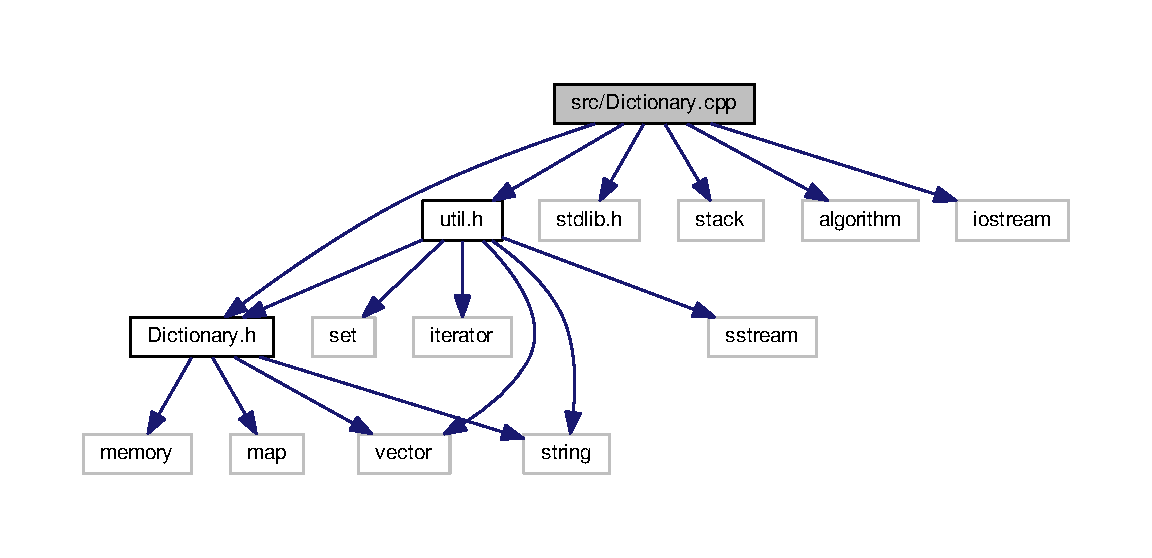
\includegraphics[width=350pt]{Dictionary_8cpp__incl}
\end{center}
\end{figure}
\subsection*{Namespaces}
\begin{DoxyCompactItemize}
\item 
\hyperlink{namespaceprdc__lzw}{prdc\-\_\-lzw}
\begin{DoxyCompactList}\small\item\em P\-R\-D\-Cで用いる\-L\-Z\-W圧縮に関する名前空間 \end{DoxyCompactList}\end{DoxyCompactItemize}


\subsection{Detailed Description}
辞書クラスの実装 \begin{DoxyDate}{Date}
2015/11/13 
\end{DoxyDate}
\begin{DoxyAuthor}{Author}
uchinosub 
\end{DoxyAuthor}


Definition in file \hyperlink{Dictionary_8cpp_source}{Dictionary.\-cpp}.


\hypertarget{Dictionary_8h}{\section{src/\-Dictionary.h File Reference}
\label{Dictionary_8h}\index{src/\-Dictionary.\-h@{src/\-Dictionary.\-h}}
}


L\-Z\-W辞書クラス定義ファイル  


{\ttfamily \#include $<$vector$>$}\\*
{\ttfamily \#include $<$string$>$}\\*
{\ttfamily \#include $<$map$>$}\\*
{\ttfamily \#include $<$memory$>$}\\*
Include dependency graph for Dictionary.\-h\-:
\nopagebreak
\begin{figure}[H]
\begin{center}
\leavevmode
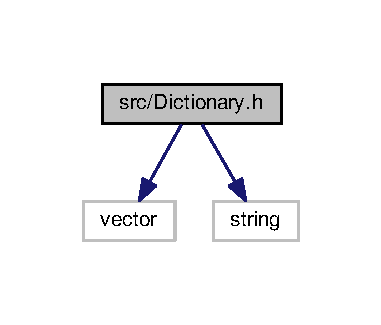
\includegraphics[width=307pt]{Dictionary_8h__incl}
\end{center}
\end{figure}
This graph shows which files directly or indirectly include this file\-:
\nopagebreak
\begin{figure}[H]
\begin{center}
\leavevmode
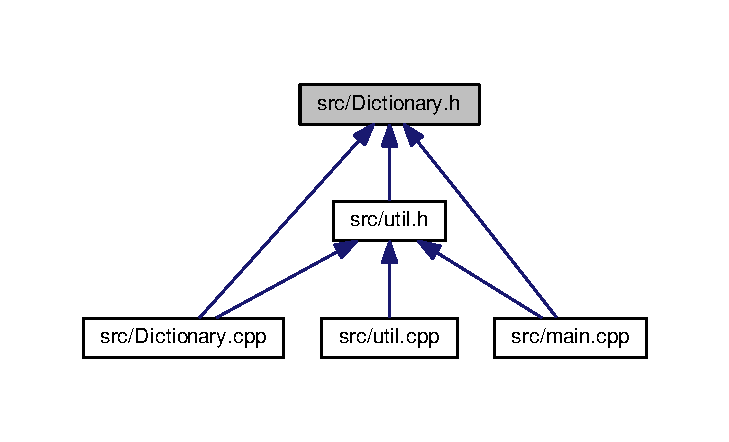
\includegraphics[width=350pt]{Dictionary_8h__dep__incl}
\end{center}
\end{figure}
\subsection*{Classes}
\begin{DoxyCompactItemize}
\item 
class \hyperlink{classprdc__lzw_1_1LzwNode}{prdc\-\_\-lzw\-::\-Lzw\-Node}
\begin{DoxyCompactList}\small\item\em L\-Z\-W辞書のノード \end{DoxyCompactList}\item 
class \hyperlink{classprdc__lzw_1_1Dictionary}{prdc\-\_\-lzw\-::\-Dictionary}
\begin{DoxyCompactList}\small\item\em L\-Z\-W辞書クラス \end{DoxyCompactList}\end{DoxyCompactItemize}
\subsection*{Namespaces}
\begin{DoxyCompactItemize}
\item 
\hyperlink{namespaceprdc__lzw}{prdc\-\_\-lzw}
\begin{DoxyCompactList}\small\item\em P\-R\-D\-Cで用いる\-L\-Z\-W圧縮に関する名前空間 \end{DoxyCompactList}\end{DoxyCompactItemize}
\subsection*{Variables}
\begin{DoxyCompactItemize}
\item 
const unsigned int \hyperlink{namespaceprdc__lzw_a32802f5b39a1712fd52ea244bed3abc6}{prdc\-\_\-lzw\-::default\-\_\-max\-\_\-dicsize} = -\/1
\begin{DoxyCompactList}\small\item\em 辞書の最大値のデフォルト値(ファイルサイスが大きく、辞書番号が50000では収まらない場合には増やす) \end{DoxyCompactList}\item 
const unsigned int \hyperlink{namespaceprdc__lzw_a563099246f7864f678056d3c7e583dbf}{prdc\-\_\-lzw\-::default\-\_\-max\-\_\-length} = -\/1
\item 
const unsigned int \hyperlink{namespaceprdc__lzw_acf8cc481fd2dd6347b910b0c0befdc84}{prdc\-\_\-lzw\-::\-D\-O\-N\-O\-T\-\_\-\-E\-D\-I\-T\-\_\-\-D\-I\-C\-T\-I\-O\-N\-A\-R\-Y} = 1
\begin{DoxyCompactList}\small\item\em フラグ処理のための定数定義 \end{DoxyCompactList}\end{DoxyCompactItemize}


\subsection{Detailed Description}
L\-Z\-W辞書クラス定義ファイル \begin{DoxyDate}{Date}
2015/11/13 
\end{DoxyDate}
\begin{DoxyAuthor}{Author}
\-: uchinosub 
\end{DoxyAuthor}


Definition in file \hyperlink{Dictionary_8h_source}{Dictionary.\-h}.


\hypertarget{main_8cpp}{\section{src/main.cpp File Reference}
\label{main_8cpp}\index{src/main.\-cpp@{src/main.\-cpp}}
}
{\ttfamily \#include $<$iostream$>$}\\*
{\ttfamily \#include $<$vector$>$}\\*
{\ttfamily \#include $<$stdio.\-h$>$}\\*
{\ttfamily \#include \char`\"{}Lzw.\-h\char`\"{}}\\*
{\ttfamily \#include \char`\"{}Dictionary.\-h\char`\"{}}\\*
Include dependency graph for main.\-cpp\-:\nopagebreak
\begin{figure}[H]
\begin{center}
\leavevmode
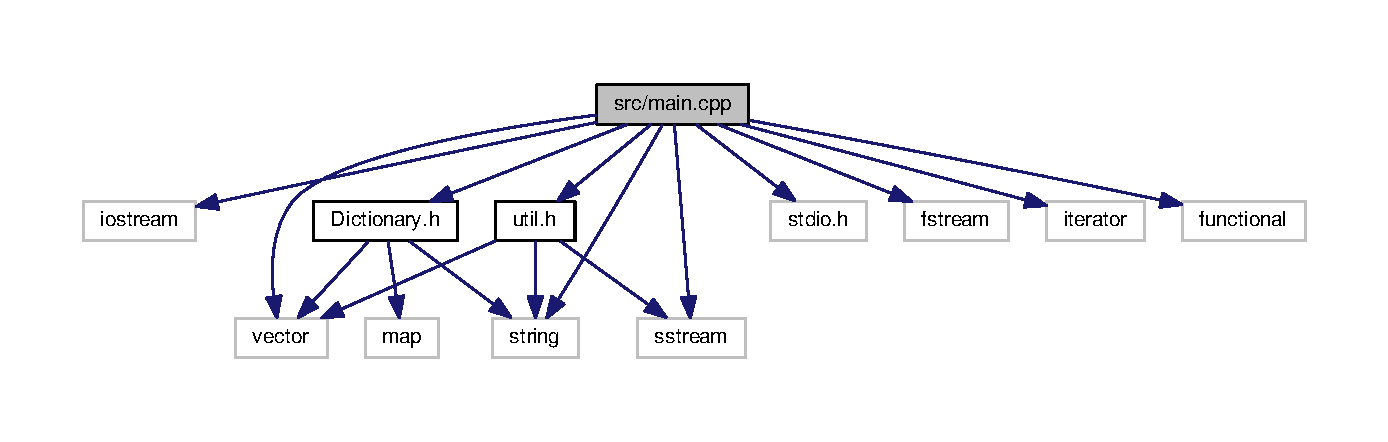
\includegraphics[width=335pt]{main_8cpp__incl}
\end{center}
\end{figure}
\subsection*{Functions}
\begin{DoxyCompactItemize}
\item 
int \hyperlink{main_8cpp_ae66f6b31b5ad750f1fe042a706a4e3d4}{main} ()
\end{DoxyCompactItemize}


\subsection{Detailed Description}
\begin{DoxyDate}{Date}
2015/11/19 
\end{DoxyDate}
\begin{DoxyAuthor}{Author}
uchinosub 
\end{DoxyAuthor}


Definition in file \hyperlink{main_8cpp_source}{main.\-cpp}.



\subsection{Function Documentation}
\hypertarget{main_8cpp_ae66f6b31b5ad750f1fe042a706a4e3d4}{\index{main.\-cpp@{main.\-cpp}!main@{main}}
\index{main@{main}!main.cpp@{main.\-cpp}}
\subsubsection[{main}]{\setlength{\rightskip}{0pt plus 5cm}int main (
\begin{DoxyParamCaption}
{}
\end{DoxyParamCaption}
)}}\label{main_8cpp_ae66f6b31b5ad750f1fe042a706a4e3d4}


Definition at line 14 of file main.\-cpp.



References prdc\-\_\-lzw\-::compress().


\input{util_8cpp}
\input{util_8h}
%--- End generated contents ---

% Index
\newpage
\phantomsection
\addcontentsline{toc}{chapter}{Index}
\printindex

\end{document}
